% Geometría del elipsoide: radios M y N, latitudes, curvatura media y su derivación desde la simetría
% Números y figuras PNG: apunte/scripts/cap14_elipsoide.py (uv run python apunte/scripts/cap14_elipsoide.py)
\chapter{Geometría del elipsoide}\label{cap:elipsoide}

\section{La idea}

\subsection{Una pregunta de campo: cuánto mide un segundo}

Imaginá que salís del ecuador caminando hacia el norte con una plomada en la mano (un hilo con
un peso en la punta, que cuelga marcando la vertical del lugar) y que te detenés cada vez que el
hilo giró un grado respecto de la dirección que tenía al salir. ¿Cuántos metros caminaste en cada tramo?
Si la Tierra fuera una esfera, todos los tramos medirían lo mismo. No es así: junto al ecuador
el tramo mide unos \(110{,}6\) km, y junto al polo, unos \(111{,}7\) km, más de un kilómetro más
(ejercicio~\ref{ex:elip-ecuador-polo}). ¿Por qué un grado de latitud mide más metros cerca del
polo que en el ecuador? Esa es la pregunta que el capítulo responde.

Mirá de perfil una naranja levemente achatada, apoyada sobre la mesa: arriba la cáscara es
casi chata, y en los costados se curva más. Donde la cáscara es chata hay que recorrer mucha
para que la dirección perpendicular a ella gire un poco; donde se curva, alcanza con poca. La
Tierra es así, apenas achatada en los polos, y la latitud se lee justamente con la
perpendicular a la superficie: por eso el grado de latitud es más largo cerca del polo, donde la
superficie es más chata.

Pensá ahora en la vertical de Buenos Aires prolongada hacia abajo, la que marcaría la plomada
si la Tierra fuera exactamente esa naranja achatada. ¿Pasa por el centro de la Tierra? En una
esfera pasaría; en la Tierra achatada, no: cruza el eje de los polos unos \(24\) km al norte
del centro. La recta que va
del punto al centro y la vertical forman ángulos distintos con el ecuador, y por eso vamos a
tener más de una latitud.

Probá también caminar \enquote{derecho} sobre una pelota y sobre un huevo. Sobre la pelota, el
suelo se curva igual hacia cualquier lado que vayas. Sobre el huevo, no: a lo largo se curva
menos que alrededor. ¿Cuántos radios hacen falta, entonces, para describir cómo se curva la
Tierra en un lugar? El capítulo~\ref{cap:curvatura} respondió en general (dos, uno por cada
dirección principal) y anticipó que en el elipsoide las curvaturas principales son \(1/M\) y
\(1/N\): \(M\) es el radio con que se curva la superficie hacia el norte, y \(N\), hacia el
este. Ahora calculamos esos radios.

Con números: en Buenos Aires, a la latitud \(\varphi\approx-34{,}6^\circ\) (el signo menos
indica el hemisferio sur), un segundo de arco de latitud, la 3600-ava parte de un grado, mide
sobre el terreno \(30{,}815\) m, y un segundo de longitud, \(25{,}481\) m. ¿Cuánto debería dar
el cociente entre los dos? Si la Tierra fuera una esfera, sería \(\cos\varphi=0{,}823136\); sobre el elipsoide
es \(0{,}826895\). La diferencia no es un error de redondeo: el elipsoide se curva distinto
a lo largo del meridiano que a lo ancho, y cada dirección tiene su propio radio. Vemos por qué
\(M\) y \(N\) son los que hacen falta y qué se gana y qué se pierde al reemplazar el elipsoide
por una esfera.

\(a\) es el radio del ecuador y \(b\), la distancia del centro a un polo, unos
\(21\) km más corta. Un \emph{meridiano} es la línea que va de polo a polo pasando por el
punto, y un \emph{paralelo}, la circunferencia horizontal que une los puntos de la misma
latitud. La latitud \(\varphi\) dice cuánto al norte o al sur del ecuador está el punto, medida
con la vertical, y la longitud \(\lambda\), cuánto al este o al oeste de un meridiano elegido
(en este capítulo, como en los dos vecinos, \(\lambda\) es siempre la longitud y nunca un
autovalor). Las otras dos latitudes, \(\psi\) y \(\beta\), miden lo mismo con otra recta en
lugar de la vertical; las presentamos en la sección~\ref{sec:latitudes}. Para trabajar en un
corte vertical que pasa por el eje, \(x'\) es la distancia horizontal del punto al eje que une
los polos y \(z\), su altura sobre el plano del ecuador. \(M\) y \(N\) son los dos radios de
curvatura de la superficie en el punto: \(M\), el del meridiano, y \(N\), el del \emph{primer
vertical}, el corte de la superficie en dirección este--oeste. \(W\) es solo una abreviatura
para no repetir una raíz que aparece en todas las fórmulas; adentro tiene la
\emph{excentricidad} \(e\), un número chico que mide cuánto se aparta la elipse de una
circunferencia (se define en la sección siguiente). La última igualdad escribe un segundo de
arco en radianes.

\subsection{Todos los meridianos son la misma elipse}

Imaginá una elipse recortada en cartón, pinchada en un alambre a lo largo de su eje corto, y
hacela girar rápido: la superficie que se ve es un \emph{elipsoide de revolución}, la forma con
que se describe la Tierra. ¿Qué cambia si te movés hacia el este sin cambiar de latitud? Nada:
la superficie que encontrás es la misma que dejaste atrás.
Esa construcción contiene dos simetrías: cualquier giro alrededor del eje polar lo deja igual,
y también la reflexión en cualquier plano que contenga al eje. De ahí se deduce casi todo sin
cuentas pesadas. Nada métrico depende de la longitud \(\lambda\): los radios, las latitudes y
la curvatura son funciones de \(\varphi\) sola, y todo se calcula en un único plano meridiano,
el corte por el eje que contiene al meridiano del punto.
La normal en un punto, la recta perpendicular a la superficie (la vertical de la plomada),
está en el plano meridiano del punto, pero no pasa por el centro, y por
eso hay más de una latitud. Y las direcciones de curvatura máxima y mínima son la del
meridiano y la del paralelo, porque la reflexión en el plano meridiano no puede preferir
ninguna otra.

\begin{idea}[La simetría elige las direcciones; las cuentas solo dan los números]
Lo que hay que calcular son los dos radios, \(M\) a lo largo del meridiano y \(N\) a lo ancho,
y ambos salen de la misma elipse.
\end{idea}

\unidadInteractiva{13_elipsoide}{Geometría del elipsoide}{Explorá: elegí el caso «elipsoide exagerado (f = 0.3)» y mové el deslizador «φ geodésica (°)» de \(0^\circ\) a \(85^\circ\). Mirá dónde corta la normal (rust) al eje polar: pasa por el centro solo en el ecuador y cerca del polo, y el tramo hasta el eje mide \(N\). Después pasá a «esfera (f = 0)» y comprobá que las tres latitudes coinciden.}

\section{Construcciones, cuentas y ejemplos}

\subsection{El elipsoide de revolución y sus parámetros}

¿Cuántos números hacen falta para fijar la forma de la Tierra en este modelo? Dos: el radio del
ecuador y la distancia del centro al polo. Todo lo demás se arma con ellos. Como la diferencia
entre los dos es chica (unos \(21\) km sobre más de \(6000\) km), conviene medirla con números que
digan directamente cuánto se aparta el elipsoide de una esfera: el \emph{achatamiento} \(f\),
la fracción del radio del ecuador que le falta al radio polar, y las \emph{excentricidades}
\(e\) y \(e'\), que valen cero en la esfera y crecen a medida que la elipse se aplana.

\begin{definicion}[Elipsoide de revolución]
Dados \(a>b>0\), el \emph{elipsoide de revolución} de semiejes \(a\) y \(b\) es la superficie
\[
  \frac{x^2}{a^2}+\frac{y^2}{a^2}+\frac{z^2}{b^2}=1 .
\]
Su \emph{achatamiento} es \(f=(a-b)/a\); su \emph{primera excentricidad} \(e\) y su
\emph{segunda excentricidad} \(e'\) se definen por
\[
  e^2=\frac{a^2-b^2}{a^2}=2f-f^2,\qquad e'^2=\frac{a^2-b^2}{b^2}=\frac{e^2}{1-e^2},
  \qquad \frac ba=\sqrt{1-e^2}=1-f .
\]
\end{definicion}

Con \(x'=\sqrt{x^2+y^2}\), la distancia al eje polar, la ecuación queda
\(x'^2/a^2+z^2/b^2=1\): cada plano que contiene al eje corta al elipsoide en la misma elipse,
la \emph{elipse meridiana}. Esa elipse es a su vez la imagen de la circunferencia de radio
\(a\) por la afinidad que comprime la dirección \(z\) en el factor \(b/a\)
(capítulo~\ref{cap:afines}); esa lectura reaparece en la latitud reducida.

Para hacer cuentas hace falta elegir un elipsoide concreto. GRS80 es uno con medidas acordadas
internacionalmente para representar la Tierra entera; el resultado que sigue da sus números y
los compara con otro de uso común, casi idéntico.

\begin{resultado}[Parámetros del elipsoide GRS80]
\(a=6\,378\,137\) m y \(1/f=298{,}257222101\). De ahí \(f=0{,}003352810681\),
\(b=6\,356\,752{,}3141\) m, \(a-b=21\,384{,}686\) m, \(e^2=0{,}0066943800\),
\(e'^2=0{,}0067394968\) y \(b/a=0{,}9966471893\). El elipsoide WGS84 tiene el mismo \(a\) y
\(1/f=298{,}257223563\): su \(b\) es \(0{,}105\) mm más largo, y en la latitud de Buenos Aires
sus \(M\) y \(N\) difieren de los de GRS80 en \(0{,}11\) mm y \(0{,}03\) mm. Para todo lo que
sigue, los dos son el mismo elipsoide; los números del capítulo son de GRS80.
\end{resultado}

\subsection{La normal, la latitud y el gran normal}

Colgá una plomada y mirá el hilo: marca la vertical del lugar. Si la Tierra fuera exactamente
un elipsoide, sin montañas ni diferencias de densidad, ese hilo sería perpendicular a la
superficie. ¿Qué ángulo forma con el plano del ecuador? Ese ángulo es el que se usa como
latitud, porque es el que se puede observar en el lugar.

La \emph{latitud geodésica} \(\varphi\) de un punto \(P\) del elipsoide es el ángulo entre la
normal al elipsoide en \(P\) y el plano del ecuador. Es la latitud que materializa la
vertical idealizada del lugar, y la que usan los sistemas oficiales de coordenadas. Para ubicar \(P\) a
partir de \(\varphi\) alcanza con trabajar en el plano meridiano: el problema es encontrar
el punto de la elipse donde la perpendicular tiene una inclinación dada.

\begin{proposicion}[El punto de latitud geodésica \(\varphi\)]\label{prop:elip-punto}
El punto de la elipse meridiana cuya normal forma el ángulo \(\varphi\) con el ecuador es
\[
  x'=N\cos\varphi,\qquad z=N(1-e^2)\sin\varphi,
  \qquad\text{con}\quad N=\frac{a}{\sqrt{1-e^2\sin^2\varphi}}=\frac aW .
\]
Con la longitud \(\lambda\), la parametrización del elipsoide es
\[
  r(\varphi,\lambda)=\bigl(N\cos\varphi\cos\lambda,\ N\cos\varphi\sin\lambda,\ N(1-e^2)\sin\varphi\bigr).
\]
\end{proposicion}

\begin{demostracion}
La elipse es la curva de nivel \(1\) de la función \(F(x',z)=x'^2/a^2+z^2/b^2\), y su gradiente
\(\nabla F=(2x'/a^2,\ 2z/b^2)\) es perpendicular a ella (capítulo~\ref{cap:formas-lineales}).
Pedir que la normal tenga la dirección \((\cos\varphi,\sin\varphi)\) es pedir
\(\dfrac{x'/a^2}{\cos\varphi}=\dfrac{z/b^2}{\sin\varphi}\), es decir,
\[
  z=\frac{b^2}{a^2}\,x'\tan\varphi=(1-e^2)\,x'\tan\varphi .
\]
Reemplazando en la elipse y usando \(b^2=a^2(1-e^2)\):
\[
  \frac{x'^2}{a^2}\bigl[1+(1-e^2)\tan^2\varphi\bigr]=1
  \quad\Longrightarrow\quad
  x'^2=\frac{a^2\cos^2\varphi}{\cos^2\varphi+(1-e^2)\sin^2\varphi}=\frac{a^2\cos^2\varphi}{1-e^2\sin^2\varphi}.
\]
Con el signo de \(\cos\varphi\) (el punto está del lado \(x'>0\)), \(x'=N\cos\varphi\), y de
la relación anterior \(z=(1-e^2)N\sin\varphi\). La longitud solo hace girar el plano
meridiano: \(x=x'\cos\lambda\), \(y=x'\sin\lambda\).
\end{demostracion}

La cantidad \(N\) tiene una lectura geométrica directa, que explica por qué la normal no
pasa por el centro. Volvamos a la plomada y prolonguemos el hilo hacia abajo, a través de la
Tierra: ¿dónde corta al eje que une los polos, y cuánto mide ese tramo?

\begin{proposicion}[El gran normal]\label{prop:elip-gran-normal}
La normal en \(P\) corta el eje polar en el punto \(z=-Ne^2\sin\varphi\), y el tramo de normal
entre \(P\) y el eje mide exactamente \(N\). Corta el plano del ecuador a distancia
\(Ne^2\cos\varphi\) del eje, y el tramo entre \(P\) y el ecuador mide \(N(1-e^2)\). En
consecuencia, la normal pasa por el centro solo en el ecuador y en los polos.
\end{proposicion}

\begin{demostracion}
Desde \(P=(N\cos\varphi,\ N(1-e^2)\sin\varphi)\), avanzar una distancia \(t\) en sentido
contrario a la normal da \(P-t(\cos\varphi,\sin\varphi)\). Con \(t=N\) se llega a
\((0,\ -Ne^2\sin\varphi)\), que está sobre el eje polar; con \(t=N(1-e^2)\) se llega a
\((Ne^2\cos\varphi,\ 0)\), sobre el ecuador. El corte con el eje es el centro solo si
\(e^2\sin\varphi=0\): en el ecuador; en el polo la normal es el propio eje.
\end{demostracion}

Por eso \(N\) se llama \emph{gran normal}: es la longitud de la normal desde el punto hasta
el eje de rotación. En Buenos Aires el hilo de la plomada, prolongado, cruza el eje \(24\,271{,}817\) m al norte del
centro (para una latitud austral, \(-Ne^2\sin\varphi>0\)) y corta el plano del ecuador a
\(35\,184{,}002\) m del eje. La figura~\ref{fig:elip-meridiana} lo muestra con un elipsoide
exagerado.

\begin{figure}[htbp]
\centering
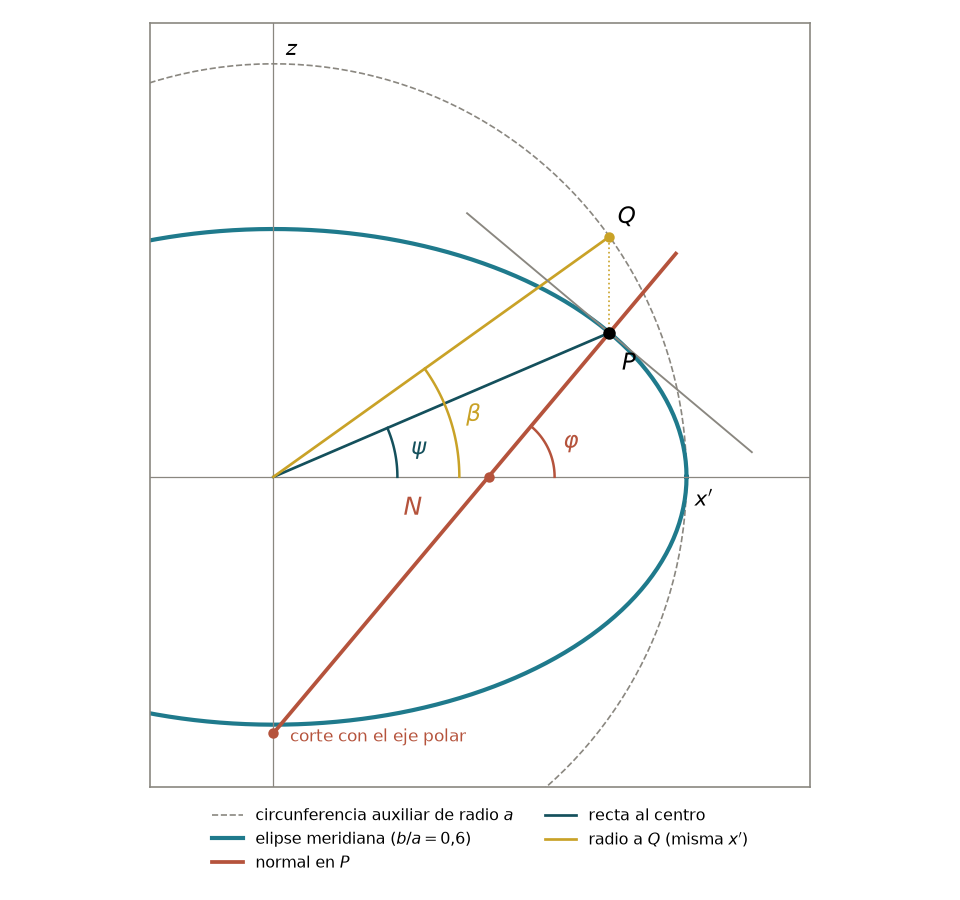
\includegraphics[width=.72\linewidth]{figuras/elipsoide/elip_meridiana.png}
\caption{Elipse meridiana exagerada (\(b/a=0{,}6\)) y un punto \(P\) de latitud geodésica
\(\varphi=50^\circ\). La normal (rust) corta el ecuador lejos del centro y el eje polar debajo
de él; el tramo hasta el eje mide \(N\approx1{,}265\,a\). La recta al centro forma la latitud
geocéntrica \(\psi\approx23{,}22^\circ\); el punto \(Q\) de la circunferencia auxiliar con la
misma \(x'\) define la reducida \(\beta\approx35{,}57^\circ\). Generada con
\texttt{apunte/scripts/cap14\_elipsoide.py}.}
\label{fig:elip-meridiana}
\end{figure}

\subsection{Tres latitudes: geodésica, geocéntrica y reducida}\label{sec:latitudes}

Parado en Buenos Aires, ¿cuánto estás \enquote{al sur} del ecuador? Depende de qué recta mires:
la vertical, la recta que va al centro de la Tierra o una tercera que facilita las cuentas.
En una esfera las tres coinciden; en el elipsoide, no.
Además de la geodésica hay otras dos maneras naturales de dar la \enquote{altura angular} de
\(P\) sobre el ecuador: la \emph{latitud geocéntrica} \(\psi\), ángulo entre la recta del
centro a \(P\) y el ecuador, y la \emph{latitud reducida} (o paramétrica) \(\beta\), ángulo del
punto \(Q\) de la circunferencia auxiliar de radio \(a\) que tiene la misma \(x'\) que \(P\).
La reducida es el parámetro de la elipse: \(x'=a\cos\beta\), \(z=b\sin\beta\).

\begin{proposicion}[Relaciones entre las tres latitudes]\label{prop:elip-latitudes}
\[
  \tan\psi=(1-e^2)\tan\varphi,\qquad
  \tan\beta=\sqrt{1-e^2}\,\tan\varphi,\qquad
  \tan^2\beta=\tan\varphi\,\tan\psi .
\]
En consecuencia \(|\psi|\le|\beta|\le|\varphi|\), con igualdad solo en el ecuador y en los
polos. La diferencia \(\varphi-\psi\) es máxima cuando \(\varphi+\psi=90^\circ\), es decir,
cuando \(\tan\varphi=1/\sqrt{1-e^2}\).
\end{proposicion}

\begin{demostracion}
Por la proposición~\ref{prop:elip-punto}, \(\tan\psi=z/x'=(1-e^2)\tan\varphi\). Para la
reducida, \(x'=a\cos\beta\) y \(z=b\sin\beta\) satisfacen la ecuación de la elipse, y
\(\tan\beta=\frac ab\,\frac z{x'}=\frac1{\sqrt{1-e^2}}(1-e^2)\tan\varphi=\sqrt{1-e^2}\tan\varphi\).
Multiplicando, \(\tan\varphi\tan\psi=(1-e^2)\tan^2\varphi=\tan^2\beta\). Como
\(0<1-e^2<\sqrt{1-e^2}<1\), las tangentes quedan ordenadas y la tangente es creciente en
\((-90^\circ,90^\circ)\). Para el máximo, con \(k=1-e^2\) y \(t=\tan\varphi\), la derivada de
\(\varphi-\arctan(k\tan\varphi)\) es \(1-\dfrac{k(1+t^2)}{1+k^2t^2}\), que se anula cuando
\(1+k^2t^2=k+kt^2\), o sea \((1-k)(1-kt^2)=0\) y \(t^2=1/k\). Ahí
\(\tan\psi=kt=\sqrt k=1/t\), de modo que \(\tan\psi=\cot\varphi\) y \(\varphi+\psi=90^\circ\).
\end{demostracion}

En el elipsoide terrestre que usamos, la máxima diferencia geodésica--geocéntrica es \(11{,}545'\) (unos \(692{,}7''\)) y
ocurre en \(\varphi=45{,}0962^\circ\); la geodésica--reducida llega a \(5{,}773'\) en
\(45{,}0481^\circ\) (figura~\ref{fig:elip-latitudes}). En Buenos Aires,
\(\psi=-34{,}420332^\circ\) y \(\beta=-34{,}510112^\circ\): la recta al centro está
\(10{,}780'\) más cerca del ecuador que la normal. A \(30{,}8\) m por segundo de latitud,
confundir las dos latitudes desplaza un punto unos \(20\) km.

\begin{figure}[htbp]
\centering
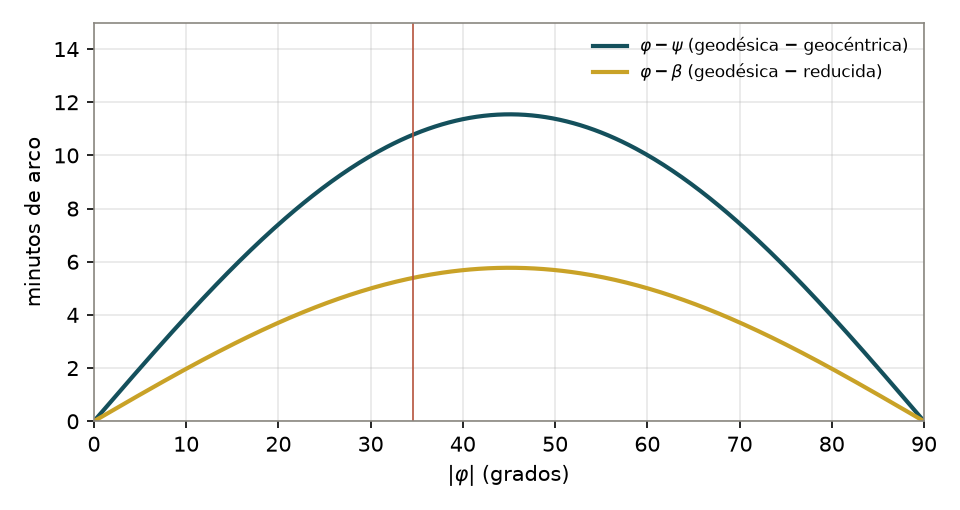
\includegraphics[width=.72\linewidth]{figuras/elipsoide/elip_latitudes.png}
\caption{Diferencias \(\varphi-\psi\) y \(\varphi-\beta\), en minutos de arco, en GRS80. Se
anulan en el ecuador y en el polo y son máximas cerca de \(45^\circ\); la recta vertical marca
la latitud de Buenos Aires.}
\label{fig:elip-latitudes}
\end{figure}

\begin{ejemplo}[Un elipsoide de juguete: \(a=5\), \(b=4\)]\label{ej:elip-juguete}
Con números chicos todo se hace a mano. \(e^2=1-16/25=0{,}36\), \(e'^2=0{,}36/0{,}64=0{,}5625\),
\(f=0{,}2\). En \(\varphi=45^\circ\), \(\sin^2\varphi=\tfrac12\) y
\(W^2=1-0{,}18=0{,}82\), \(W=0{,}905539\):
\[
  N=\frac5{0{,}905539}=5{,}521576,\qquad
  x'=N\cos45^\circ=3{,}904344,\qquad
  z=0{,}64\,N\sin45^\circ=2{,}498780 .
\]
Control: \(x'^2/25+z^2/16=0{,}609756+0{,}390244=1\). La normal corta el eje polar en
\(z=-Ne^2\sin45^\circ=-1{,}405564\) y el ecuador en \(x'=1{,}405564\). Las latitudes:
\(\tan\psi=0{,}64\), \(\psi=32{,}6192^\circ\); \(\tan\beta=0{,}8\), \(\beta=38{,}6598^\circ\); y
\(\tan^2\beta=0{,}64=\tan45^\circ\tan\psi\). Con un achatamiento así, la recta al centro y la
normal difieren en más de \(12^\circ\).
\end{ejemplo}

\subsection{Radios de curvatura \texorpdfstring{\(M\)}{M} y \texorpdfstring{\(N\)}{N}}\label{sec:radios-MN}

Volvé a la naranja achatada vista de perfil y a la caminata con la plomada. Para que la
vertical gire un grado hay que recorrer más cáscara donde es chata y menos donde se curva: el
largo de ese recorrido, por cada radián que gira la vertical, es justamente el radio de
curvatura. Esta sección lo calcula en las dos direcciones que importan, hacia el norte y hacia
el este.

\paragraph{El meridiano.} La curvatura de una curva plana, \(\kappa\) (se lee
\enquote{kappa}), es la rapidez con que gira su
tangente por unidad de longitud recorrida, \(\kappa=d\theta/ds\), y el radio de curvatura es
\(1/\kappa\). En la elipse meridiana el ángulo de la tangente está atado a la latitud: la
tangente es perpendicular a la normal, de modo que \(\theta=\varphi+90^\circ\) y
\(d\theta=d\varphi\). Solo falta saber cuánto se avanza por cada \(d\varphi\).

\begin{proposicion}[Radio de curvatura del meridiano]\label{prop:elip-M}
Sobre la elipse meridiana parametrizada por la latitud geodésica,
\[
  \frac{d}{d\varphi}\bigl(x',z\bigr)=M\,(-\sin\varphi,\ \cos\varphi),
  \qquad
  M=\frac{a(1-e^2)}{(1-e^2\sin^2\varphi)^{3/2}}=\frac{a(1-e^2)}{W^3}.
\]
En consecuencia \(ds=M\,d\varphi\) y la curvatura del meridiano es \(1/M\): \(M\) es el radio
de la circunferencia osculadora de la elipse meridiana en \(P\).
\end{proposicion}

En palabras: cuando la latitud aumenta en \(d\varphi\), el punto avanza sobre el meridiano una
distancia \(ds=M\,d\varphi\), y \(M\) es el radio de la circunferencia que mejor se pega a la
elipse en ese punto (la osculadora del capítulo~\ref{cap:curvatura}).

\begin{demostracion}
De \(N=aW^{-1}\) y \(dW/d\varphi=-e^2\sin\varphi\cos\varphi/W\) sale
\(dN/d\varphi=ae^2\sin\varphi\cos\varphi/W^3\). Entonces
\[
\begin{aligned}
  \frac{d(N\cos\varphi)}{d\varphi}
  &=\frac{ae^2\sin\varphi\cos^2\varphi}{W^3}-\frac{a\sin\varphi}{W}\\
  &=\frac{a\sin\varphi\,(e^2\cos^2\varphi-1+e^2\sin^2\varphi)}{W^3}
  =-\frac{a(1-e^2)}{W^3}\sin\varphi ,
\end{aligned}
\]
\[
\begin{aligned}
  \frac{d\bigl(N(1-e^2)\sin\varphi\bigr)}{d\varphi}
  &=(1-e^2)\Bigl[\frac{ae^2\sin^2\varphi\cos\varphi}{W^3}+\frac{a\cos\varphi}{W}\Bigr]\\
  &=(1-e^2)\frac{a\cos\varphi\,(e^2\sin^2\varphi+1-e^2\sin^2\varphi)}{W^3}
  =\frac{a(1-e^2)}{W^3}\cos\varphi .
\end{aligned}
\]
El vector derivado tiene largo \(M\), así que \(ds/d\varphi=M\) y
\(\kappa=d\theta/ds=(d\theta/d\varphi)/(ds/d\varphi)=1/M\).
\end{demostracion}

La cuenta se puede controlar por otro camino: la fórmula de la curvatura de una curva
implícita aplicada a \(x'^2/a^2+z^2/b^2=1\) en Buenos Aires da un radio de
\(6\,356\,008{,}141\) m, el mismo \(M\).

\paragraph{La primera forma fundamental.} ¿Y si el paso no es hacia el norte sino en
cualquier dirección? Hace falta una regla que convierta un cambio chico de latitud y de
longitud en metros sobre la superficie: es la primera forma fundamental del
capítulo~\ref{cap:curvatura}. En tres dimensiones, derivando
\(r(\varphi,\lambda)\) de la proposición~\ref{prop:elip-punto} y usando la
proposición~\ref{prop:elip-M},
\[
  r_\varphi=M\,(-\sin\varphi\cos\lambda,\ -\sin\varphi\sin\lambda,\ \cos\varphi),\qquad
  r_\lambda=N\cos\varphi\,(-\sin\lambda,\ \cos\lambda,\ 0).
\]
Aquí \(r_\varphi\) y \(r_\lambda\) son las derivadas de \(r\) respecto de la latitud y de la
longitud: las flechas que dicen hacia dónde y cuánto se mueve el punto al cambiar cada
coordenada, la primera hacia el norte y la segunda hacia el este.
Los dos son perpendiculares entre sí y a \(n=(\cos\varphi\cos\lambda,\ \cos\varphi\sin\lambda,\
\sin\varphi)\), la normal de latitud \(\varphi\). Con la notación de la
sección~\ref{sec:metrica} (capítulo~\ref{cap:derivada}), \(E=M^2\), \(F=0\),
\(G=N^2\cos^2\varphi\) y
\[
  \boxed{\ ds^2=M^2\,d\varphi^2+N^2\cos^2\varphi\,d\lambda^2\ }.
\]
La esfera de radio \(R\) es el caso \(M=N=R\). La fórmula dice cómo convertir diferencias de
coordenadas en metros: un \(d\varphi\) mide \(M\,d\varphi\) sobre el meridiano y un
\(d\lambda\) mide \(N\cos\varphi\,d\lambda\) sobre el paralelo, que es una circunferencia de
radio \(x'=N\cos\varphi\).

\paragraph{El primer vertical y las curvaturas principales.} Parado en el punto, cortá
mentalmente la superficie con un plano vertical que contenga a la normal y apunte al este: la
curva que queda es el \emph{primer vertical}. ¿Por qué el norte y el este, y no otras dos
direcciones? En general las direcciones
principales son autovectores del operador de forma (sección~\ref{sec:curvaturas-principales});
en el elipsoide no hace falta diagonalizar nada: la simetría las elige.

\begin{proposicion}[Curvaturas principales del elipsoide]\label{prop:elip-principales}
En todo punto del elipsoide que no sea un polo, las direcciones principales son la del
meridiano y la del paralelo, y las curvaturas principales son
\[
  k_1=\frac1M\quad\text{(meridiano)},\qquad k_2=\frac1N\quad\text{(primer vertical)},
  \qquad k_1\ge k_2 .
\]
Los meridianos y los paralelos son líneas de curvatura.
\end{proposicion}

\begin{demostracion}
\emph{Las direcciones, por simetría.} La reflexión en el plano meridiano de \(P\) lleva el
elipsoide en sí mismo, deja fijos \(P\) y su normal, y en coordenadas cambia
\(\lambda-\lambda_P\) por \(\lambda_P-\lambda\): en el plano tangente manda
\((d\varphi,d\lambda)\) a \((d\varphi,-d\lambda)\). Como es una isometría que respeta la
normal, la segunda forma fundamental
\(\mathrm{II}=h_{11}\,d\varphi^2+2h_{12}\,d\varphi\,d\lambda+h_{22}\,d\lambda^2\) toma el mismo
valor en los dos vectores, y eso obliga a \(h_{12}=0\). La primera forma ya era diagonal
(\(F=0\)), de modo que las dos formas son diagonales en las direcciones de \(r_\varphi\) y
\(r_\lambda\): esas son las direcciones principales.

\emph{El meridiano.} El plano meridiano contiene a la normal, así que el meridiano es una
sección normal; su curvatura, \(1/M\) por la proposición~\ref{prop:elip-M}, es la curvatura
normal en esa dirección.

\emph{El paralelo.} El paralelo de \(P\) es una circunferencia de radio \(N\cos\varphi\), con
curvatura \(1/(N\cos\varphi)\) y normal principal horizontal, apuntando al eje. Esa
dirección forma el ángulo \(\varphi\) con la normal al elipsoide, y por el teorema de
Meusnier (sección~\ref{sec:curvaturas-principales}) la curvatura normal en la dirección este
es \(\cos\varphi/(N\cos\varphi)=1/N\).

\emph{El orden.} \(N/M=W^2/(1-e^2)=1+e'^2\cos^2\varphi\ge1\), con igualdad solo en los polos.
\end{demostracion}

\paragraph{Una esfera tangente a lo largo de todo el paralelo.} El cálculo de \(1/N\) tiene
una lectura sin fórmulas. Por la simetría de revolución, las normales en todos los puntos del
paralelo de \(P\) pasan por el mismo punto del eje, \(z=-Ne^2\sin\varphi\), y miden \(N\)
hasta él (proposición~\ref{prop:elip-gran-normal}). La esfera con centro en ese punto y radio
\(N\) es entonces tangente al elipsoide a lo largo de todo el paralelo: comparte la curva y la
normal en cada uno de sus puntos, y por lo tanto la curvatura normal en la dirección del
paralelo. Esa curvatura es la de la esfera, \(1/N\). Por eso la sección normal este--oeste se
llama \emph{primer vertical} y su radio coincide con el gran normal.

\animacion{05_elipsoide_euler_meusnier}{Euler y Meusnier sobre el elipsoide}{Mirá cómo varía el radio de la sección normal al girar su acimut entre el meridiano y el primer vertical.}

\begin{figure}[htbp]
\centering
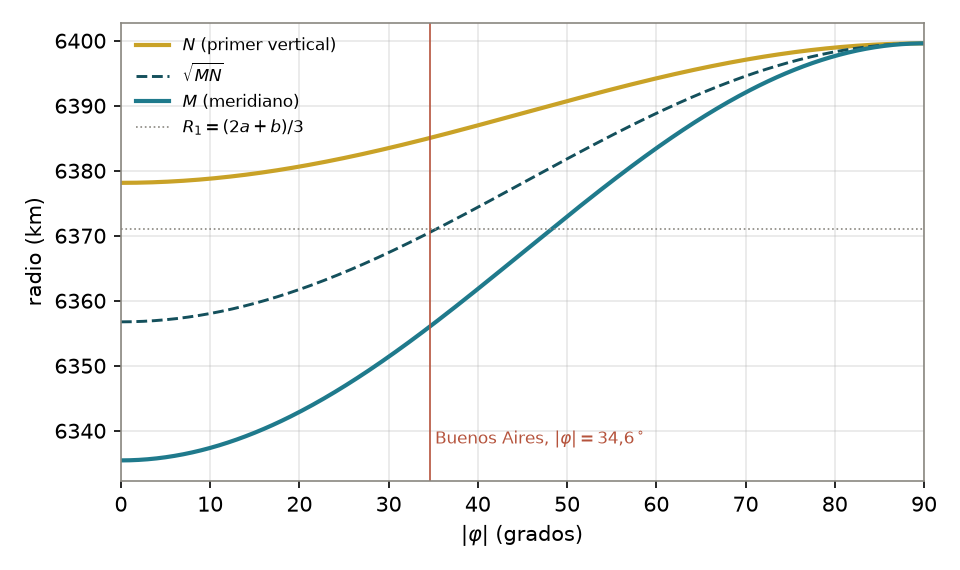
\includegraphics[width=.75\linewidth]{figuras/elipsoide/elip_radios.png}
\caption{Radios \(M\) y \(N\) y su media geométrica \(\sqrt{MN}\) en GRS80, en función de la
latitud. En el ecuador \(M=b^2/a\) es mínimo y \(N=a\); en el polo los dos valen \(a^2/b\). La
línea punteada es el radio medio \(R_1=(2a+b)/3\), que no depende de la latitud.}
\label{fig:elip-radios}
\end{figure}

\begin{ejemplo}[Valores de control en GRS80]\label{ej:elip-control}
Con \(a=6\,378\,137\) m y \(e^2=0{,}00669438\):

{\small
\begin{center}
\begin{tabular}{l rrrr}
\toprule
 & \(\varphi=0^\circ\) & \(\varphi=45^\circ\) & \(\varphi=-34{,}6^\circ\) & \(\varphi=90^\circ\)\\
\midrule
\(M\) (m) & 6\,335\,439{,}327 & 6\,367\,381{,}816 & 6\,356\,008{,}141 & 6\,399\,593{,}626\\
\(N\) (m) & 6\,378\,137{,}000 & 6\,388\,838{,}290 & 6\,385\,032{,}023 & 6\,399\,593{,}626\\
\(x'=N\cos\varphi\) (m) & 6\,378\,137{,}000 & 4\,517\,590{,}879 & 5\,255\,752{,}072 & 0\\
\(z\) (m) & 0 & 4\,487\,348{,}409 & \(-3\,601\,428{,}679\) & 6\,356\,752{,}314\\
\(\psi\) & \(0^\circ\) & \(44{,}807577^\circ\) & \(-34{,}420332^\circ\) & \(90^\circ\)\\
\(\beta\) & \(0^\circ\) & \(44{,}903788^\circ\) & \(-34{,}510112^\circ\) & \(90^\circ\)\\
\(\sqrt{MN}\) (m) & 6\,356\,752{,}314 & 6\,378\,101{,}030 & 6\,370\,503{,}553 & 6\,399\,593{,}626\\
\bottomrule
\end{tabular}
\end{center}
}

En cada columna \(x'^2/a^2+z^2/b^2=1\) con error de redondeo de máquina. En el ecuador,
\(M=a(1-e^2)=b^2/a\) y \(N-M=ae^2=42\,697{,}673\) m; en el polo, \(M=N=a/\sqrt{1-e^2}=a^2/b\);
en el ecuador \(\sqrt{MN}=b\). En Buenos Aires,
\(N/M=1{,}00456637=1+e'^2\cos^2\varphi\): el elipsoide se curva allí un \(0{,}46\)\,\% más a lo
largo del meridiano que a lo ancho.
\end{ejemplo}

\subsection{Radio medio de Gauss y curvatura media}

Si hubiera que reemplazar el elipsoide, cerca de un punto, por una sola esfera, ¿qué radio
habría que elegir: \(M\), \(N\) o algo intermedio? Para responder, resumimos las dos
curvaturas en un solo número.
Con las curvaturas principales se arman los dos invariantes del capítulo~\ref{cap:curvatura}:
\[
  K=k_1k_2=\frac1{MN}\quad\text{(curvatura de Gauss)},\qquad
  H=\frac{k_1+k_2}2=\frac12\Bigl(\frac1M+\frac1N\Bigr)\quad\text{(curvatura media)} .
\]
El \emph{radio medio de Gauss} es \(R=1/\sqrt K=\sqrt{MN}\): el radio de la esfera que tiene,
en ese punto, la misma curvatura de Gauss que el elipsoide. Una dirección sobre el terreno se
da con su \emph{acimut} \(\alpha\), el ángulo que forma con el norte, contado en sentido
horario. Entre las secciones normales, los cortes por planos que contienen a la normal, la
fórmula de Euler da el radio \(\rho(\alpha)\) de la sección en cada dirección:
\[
  \frac1{\rho(\alpha)}=\frac{\cos^2\alpha}M+\frac{\sin^2\alpha}N .
\]

\begin{proposicion}[\(\sqrt{MN}\) es el radio promedio de las secciones normales]\label{prop:elip-media}
El promedio de \(\rho(\alpha)\) sobre todos los acimutes es \(\sqrt{MN}\); el promedio de la
curvatura \(1/\rho(\alpha)\) es \(H\), y \(1/H=2MN/(M+N)=\rho(45^\circ)\).
\end{proposicion}

\begin{demostracion}
Por simetría alcanza con el primer cuadrante. Dividiendo numerador y denominador por
\(\cos^2\alpha\) y con \(t=\tan\alpha\), \(dt=d\alpha/\cos^2\alpha\):
\[
  \int_0^{\pi/2}\frac{d\alpha}{\cos^2\alpha/M+\sin^2\alpha/N}
  =\int_0^\infty\frac{dt}{1/M+t^2/N}
  =N\int_0^\infty\frac{dt}{N/M+t^2}
  =N\,\frac{\pi/2}{\sqrt{N/M}}=\frac\pi2\sqrt{MN},
\]
y dividiendo por \(\pi/2\) queda el promedio. Para la curvatura, el promedio de
\(\cos^2\alpha\) y de \(\sin^2\alpha\) es \(\tfrac12\), así que el de \(1/\rho\) es \(H\); en
\(\alpha=45^\circ\) los dos pesos valen \(\tfrac12\) y \(1/\rho(45^\circ)=H\).
\end{demostracion}

Los tres promedios de \(M\) y \(N\) aparecen así con significado propio: la media armónica
\(2MN/(M+N)=1/H\), la geométrica \(\sqrt{MN}=1/\sqrt K\) y la aritmética \((M+N)/2\). En
Buenos Aires valen \(6\,370\,487{,}024\) m, \(6\,370\,503{,}553\) m y \(6\,370\,520{,}082\) m, y
\(K=2{,}464067\cdot10^{-14}\) m\(^{-2}\). La integral numérica de \(\rho(\alpha)\) en la vuelta
completa reproduce \(\sqrt{MN}\) al nanómetro.

\paragraph{La esfera local.} Entre todas las esferas tangentes al elipsoide en \(P\), la de
radio \(\sqrt{MN}\) es la que tiene su misma curvatura de Gauss, y la que mejor reemplaza al
radio de las secciones normales promediado en todas las direcciones
(figura~\ref{fig:elip-esfera-local}). Lo que depende de la superficie solo a través de
\(K\), como el exceso de un triángulo pequeño (sección~\ref{sec:exceso-esferico}), se calcula
igual sobre esa esfera; por eso es la esfera natural para aplicar, en un entorno del punto, la
trigonometría esférica del capítulo~\ref{cap:esfera}. Lo que no reproduce es la métrica dirección por dirección:
la aplicación topográfica mide cuánto.

\begin{figure}[htbp]
\centering
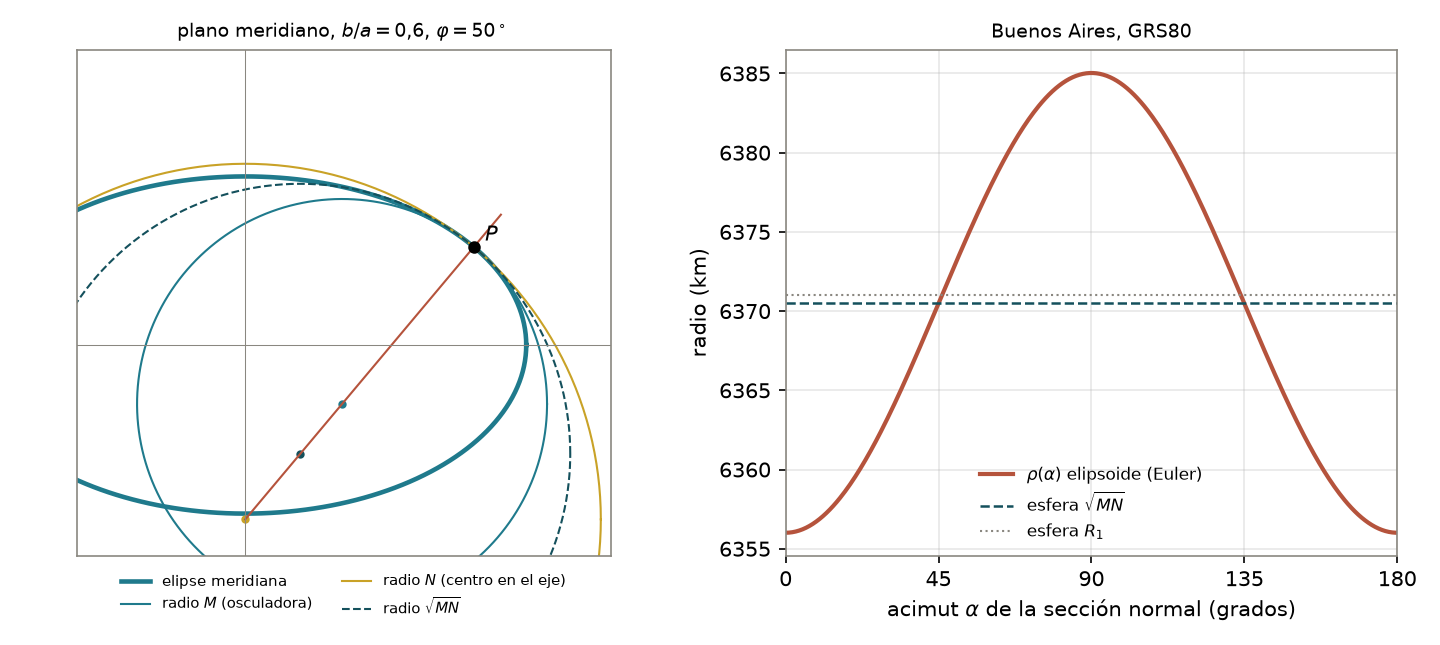
\includegraphics[width=\linewidth]{figuras/elipsoide/elip_esfera_local.png}
\caption{La esfera local. Izquierda: en la elipse exagerada, las circunferencias tangentes en
\(P\) de radios \(M\) (osculadora del meridiano), \(N\) (con centro en el eje polar, sobre la
normal) y \(\sqrt{MN}\). Derecha: radio \(\rho(\alpha)\) de la sección normal en Buenos Aires
(GRS80) en función del acimut, de \(M\) en el meridiano a \(N\) en el primer vertical; la
esfera de radio \(\sqrt{MN}\) lo corta cerca de \(45^\circ\) y de \(135^\circ\).}
\label{fig:elip-esfera-local}
\end{figure}

\unidadInteractiva{13_elipsoide}{Geometría del elipsoide}{Verificá: con el caso «elipsoide de juguete a = 5, b = 4» y el deslizador «φ geodésica (°)» en \(45^\circ\), comprobá en los números vivos los valores del ejemplo~\ref{ej:elip-juguete}: \(M=4{,}3095\), \(N=5{,}5216\), \(\psi\approx32^\circ37'\), \(\beta\approx38^\circ40'\). Después elegí «GRS80 (f = 1/298.257)», llevá \(\varphi\) a \(45^\circ\) y verificá que \(1'\) de \(\varphi\) mide \(1\,852{,}20\) m, \(1'\) de \(\lambda\) mide \(1\,314{,}11\) m y \(N-M=21\,456{,}47\) m.}

\section{En profundidad}

\subsection{Longitud del arco de meridiano}

Como \(ds=M\,d\varphi\) sobre el meridiano, la distancia desde el ecuador hasta la latitud
\(\varphi\) es
\[
  S(\varphi)=\int_0^{\varphi}M\,d\varphi=a(1-e^2)\int_0^{\varphi}\bigl(1-e^2\sin^2t\bigr)^{-3/2}dt ,
\]
una integral sin primitiva elemental. Hay dos caminos: integrarla numéricamente (por ejemplo,
con la función \texttt{quad} del módulo \texttt{scipy.integrate}) o desarrollar el integrando en serie, que deja una fórmula
cerrada con coeficientes que se calculan una vez por elipsoide.

\paragraph{Serie binomial.} Para \(|x|<1\),
\((1-x)^{-3/2}=\sum_{n\ge0}c_nx^n\) con
\(c_n=\dfrac{(2n+1)!}{(2^n\,n!)^2}\): \(1,\ \tfrac32,\ \tfrac{15}8,\ \tfrac{35}{16},\
\tfrac{315}{128},\dots\) Con \(x=e^2\sin^2t\) quedan potencias pares del seno, todas con
coeficiente positivo.

\paragraph{Potencias del seno como cosenos de ángulos múltiples.} Desarrollando
\(\sin t=(e^{it}-e^{-it})/(2i)\) por el binomio,
\[
  \sin^{2n}t=\frac1{4^n}\Bigl[\binom{2n}{n}+2\sum_{k=1}^{n}(-1)^k\binom{2n}{n-k}\cos2kt\Bigr],
\]
por ejemplo \(\sin^2t=\tfrac12(1-\cos2t)\) y \(\sin^4t=\tfrac18(3-4\cos2t+\cos4t)\). Los
cosenos sí se integran.

\begin{resultado}[Arco de meridiano en serie]
Agrupando hasta \(e^8\),
\[
  S(\varphi)=a(1-e^2)\Bigl[A\varphi+\frac B2\sin2\varphi+\frac C4\sin4\varphi
  +\frac D6\sin6\varphi+\frac E8\sin8\varphi\Bigr],
\]
\[
\begin{aligned}
  A&=1+\tfrac34e^2+\tfrac{45}{64}e^4+\tfrac{175}{256}e^6+\tfrac{11025}{16384}e^8, &
  B&=-\bigl(\tfrac34e^2+\tfrac{15}{16}e^4+\tfrac{525}{512}e^6+\tfrac{2205}{2048}e^8\bigr),\\
  C&=\tfrac{15}{64}e^4+\tfrac{105}{256}e^6+\tfrac{2205}{4096}e^8, &
  D&=-\bigl(\tfrac{35}{512}e^6+\tfrac{315}{2048}e^8\bigr),\qquad
  E=\tfrac{315}{16384}e^8 .
\end{aligned}
\]
En GRS80: \(A=1{,}0050525018\), \(B=-5{,}0631086\cdot10^{-3}\),
\(C=1{,}0627582\cdot10^{-5}\), \(D=-2{,}08172\cdot10^{-8}\), \(E=3{,}861\cdot10^{-11}\).
\end{resultado}

Controles contra la integral numérica: del ecuador a \(45^\circ\),
\(S=4\,984\,944{,}378\) m; del ecuador a \(-34{,}6^\circ\), \(S=-3\,830\,218{,}134\) m (el signo
indica el hemisferio sur); el cuadrante de meridiano, \(10\,001\,965{,}729\) m. En los tres casos
la serie coincide con la integral en menos de \(0{,}1\) mm. Cuánto aporta cada término se ve
truncando: hasta Buenos Aires, quedarse con \(A\varphi\) solo erra en \(-14\,982{,}024\) m;
agregar \(B\) deja \(11{,}186\) m; agregar \(C\), \(0{,}010\) m.

\paragraph{Arco de paralelo.} El paralelo es una circunferencia de radio \(N\cos\varphi\), de
modo que el arco entre dos longitudes es exactamente \(S_\lambda=N\cos\varphi\,\Delta\lambda\).
Clavá dos chinches sobre una pelota, a la misma altura pero lejos del ecuador, y tensá una
cuerda entre ellas: ¿la cuerda sigue el paralelo? No: se va un poco hacia el polo, porque por
ahí el camino es más corto. Esa línea más corta sobre la superficie, la que sigue la cuerda
tensa, se llama \emph{geodésica}. En el elipsoide pasa lo mismo: el arco de paralelo no es la
línea más corta entre sus extremos, la geodésica que los une se desvía
levemente hacia el polo, y para \(10\) km en Buenos Aires es \(0{,}49\) mm más corta.

\subsection{Aplicación topográfica: un segundo y una base de 10 km en Buenos Aires}

La situación: se conocen la latitud y la longitud de un punto en Buenos Aires y hay que saber
cuántos metros representa un segundo de cada coordenada, y qué coordenadas tiene un punto
ubicado a \(10\) km hacia el norte o hacia el este. Ese segmento de \(10\) km, de largo
conocido y usado como referencia, es lo que en el ejemplo llamamos \emph{base}. La tentación es
hacer las cuentas sobre una esfera, que tiene fórmulas más simples; el ejemplo mide cuánto se
pierde. Los errores aparecen en \emph{partes por millón}: un error de una parte por millón es un
milímetro por kilómetro. Al final, las cuentas cerradas se comparan con un cálculo
independiente, con un margen de error aceptado de un milímetro.

\begin{ejemplo}[Radios, segundos y bases en Buenos Aires]\label{ej:elip-ba}
En \(\varphi=-34{,}6^\circ\), GRS80:
\[
  M=6\,356\,008{,}141\ \text{m},\qquad N=6\,385\,032{,}023\ \text{m},\qquad
  N\cos\varphi=5\,255\,752{,}072\ \text{m}.
\]
\textbf{Un segundo.} \(1''\) de latitud mide \(M\cdot1''=30{,}8148\) m y \(1''\) de longitud,
\(N\cos\varphi\cdot1''=25{,}4806\) m. Sobre una esfera de radio \(R_1=(2a+b)/3=6\,371\,008{,}771\)
m serían \(30{,}8875\) m y \(25{,}4246\) m: errores de \(7\) y \(6\) cm por segundo, que en
\(1'\) ya son metros.

\textbf{Diez kilómetros en segundos.} Hacia el norte, \(10\,000/M\) da \(324{,}5194''\); la
integración exacta del arco de meridiano desde \(-34{,}6^\circ\) da \(324{,}5218''\) (el radio
\(M\) disminuye al acercarse al ecuador y hace falta un poco más de ángulo), y el extremo queda
en \(\varphi_2=-34{,}509855050^\circ\). Hacia el este, sobre el paralelo,
\(\Delta\lambda=10\,000/(N\cos\varphi)=392{,}4554''=6'\,32{,}455''\).

\textbf{La misma base sobre una esfera.} Tomamos los extremos de cada base con sus
coordenadas \((\varphi,\lambda)\) y calculamos la distancia sobre una esfera, como si las
coordenadas fueran esféricas:

\begin{center}
\begin{tabular}{l rr}
\toprule
 & base hacia el norte & base hacia el este\\
\midrule
elipsoide & 10\,000{,}000 m & 10\,000{,}000 m\\
esfera de radio \(\sqrt{MN}=6\,370\,503{,}553\) m & 10\,022{,}880 m (\(+22{,}880\)) & 9\,977{,}246 m (\(-22{,}754\))\\
esfera de radio \(R_1=6\,371\,008{,}771\) m & 10\,023{,}675 m (\(+23{,}675\)) & 9\,978{,}037 m (\(-21{,}963\))\\
\bottomrule
\end{tabular}
\end{center}

Hacia el norte la esfera usa \(R\) donde el elipsoide usa \(M\), y hacia el este \(R\) donde
corresponde \(N\): los errores relativos son \(R/M-1\) y \(R/N-1\). Con \(R=\sqrt{MN}\) valen
\(+2281\) y \(-2275\) partes por millón, simétricos porque \(\sqrt{MN}/M\) y
\(\sqrt{MN}/N\) son inversos; con \(R_1\), que es un promedio global y no sabe de la latitud,
\(+2360\) y \(-2196\). Unos \(23\) m en \(10\) km: ninguna esfera sirve para convertir
diferencias de coordenadas geodésicas en distancias.

\textbf{Lo que la esfera local sí reproduce.} Las magnitudes que dependen de la curvatura y
no de la escala de las coordenadas. El apartamiento de la superficie respecto del plano
tangente a \(10\) km del punto, \(s^2/(2\rho)\), es \(7\,866{,}6\) mm hacia el norte
(\(\rho=M\)) y \(7\,830{,}8\) mm hacia el este (\(\rho=N\)); la esfera de radio \(\sqrt{MN}\) da
\(7\,848{,}7\) mm en las dos direcciones, a \(18\) mm de cada uno. La diferencia entre el arco y
la cuerda, \(s^3/(24\rho^2)\), es \(1{,}0314\) mm y \(1{,}0220\) mm, y la esfera da \(1{,}0267\)
mm: un error de cinco milésimas de milímetro.

\textbf{Control independiente.} El cálculo geodésico de \texttt{pyproj}
(\texttt{Geod(ellps='GRS80').inv}), usado solo como control, da para la base hacia el norte
\(10\,000{,}000000\) m, para \(1''\) de latitud \(30{,}814796\) m (contra \(30{,}814797\) m de
\(M\cdot1''\), que ignora la variación de \(M\) dentro del segundo), para \(1''\) de longitud
\(25{,}480605\) m, y para la base hacia el este \(9\,999{,}999514\) m: la geodésica entre los
extremos del arco de paralelo, \(0{,}49\) mm más corta que el arco. El cuadrante de meridiano
coincide con la integral numérica. Con una tolerancia declarada de \(1\) mm, todas las
fórmulas cerradas del ejemplo pasan el control.
\end{ejemplo}

\begin{atencion}[Dos esferas, dos usos]
La esfera de radio \(\sqrt{MN}\) sirve para lo que depende de la curvatura en un entorno del
punto: reducciones de arco a cuerda, apartamiento del plano tangente, exceso de triángulos
pequeños. Para pasar de diferencias de latitud y longitud a metros hay que usar \(M\) y
\(N\cos\varphi\), o la primera forma fundamental completa; ninguna esfera las reemplaza con
error menor que unas partes por mil.
\end{atencion}

\subsection{Alcance}

Todo el capítulo se apoya en la simetría de revolución. Si el elipsoide tuviera tres ejes
distintos, los meridianos dejarían de ser la misma elipse, \(M\) y \(N\) dependerían también
de la longitud y las direcciones principales ya no estarían fijadas de antemano: habría que
hallarlas como autovectores, como en el capítulo~\ref{cap:curvatura}. Las proyecciones que
llevan este elipsoide al plano se desarrollan en el complemento~\ref{cap:conformes}, y la
manera de atarlo a puntos concretos de la Tierra, en el complemento~\ref{cap:marcos}.
El capítulo~\ref{cap:esfera} toma la esfera local de radio \(\sqrt{MN}\) y resuelve triángulos
sobre ella.

\section{Ejercicios con solución}

\begin{ejercicio}\label{ex:elip-ecuador-polo}
En GRS80, calculá \(M\) y \(N\) en el ecuador y en el polo, verificá que \(N-M=ae^2\) en el
ecuador y compará la longitud de \(1^\circ\) de meridiano junto al ecuador y junto al polo.
¿Dónde es más largo un grado de latitud, y por qué eso indica que la Tierra está achatada en
los polos?
\end{ejercicio}
\solucion{En el ecuador \(M=b^2/a=6\,335\,439{,}327\) m y \(N=a=6\,378\,137\) m, con
\(N-M=a-a(1-e^2)=ae^2=42\,697{,}673\) m. En el polo \(M=N=a^2/b=6\,399\,593{,}626\) m. Integrando
\(M\), el grado de \(0^\circ\) a \(1^\circ\) mide \(110\,574{,}389\) m y el de \(89^\circ\) a
\(90^\circ\), \(111\,693{,}865\) m. El grado de latitud es más largo cerca del polo porque allí
el meridiano es menos curvo (radio mayor): la superficie está más aplanada en los polos.}

\begin{ejercicio}\label{ex:elip-geocentrica}
Un punto de GRS80 tiene latitud geocéntrica \(\psi=30^\circ\). Hallá su latitud geodésica y
su latitud reducida, y verificá la relación \(\tan^2\beta=\tan\varphi\tan\psi\).
\end{ejercicio}
\solucion{\(\tan\varphi=\tan30^\circ/(1-e^2)\) da \(\varphi=30{,}166924^\circ\), \(10{,}015'\)
más que \(\psi\). \(\tan\beta=\sqrt{1-e^2}\tan\varphi\) da \(\beta=30{,}083392^\circ\), a
\(5{,}004'\) de \(\psi\): la reducida queda casi en el medio, como corresponde a una media
geométrica de las tangentes. \(\tan^2\beta=0{,}3355798323=\tan\varphi\tan\psi\).}

\begin{ejercicio}\label{ex:elip-euler}
En Buenos Aires (GRS80), calculá el radio de la sección normal en los acimutes \(30^\circ\),
\(45^\circ\) y \(60^\circ\). Mostrá que \(\rho(45^\circ)=2MN/(M+N)\) y comparalo con
\(\sqrt{MN}\).
\end{ejercicio}
\solucion{Con la fórmula de Euler y los \(M\), \(N\) del ejemplo~\ref{ej:elip-ba}:
\(\rho(30^\circ)=6\,363\,239{,}346\) m, \(\rho(45^\circ)=6\,370\,487{,}024\) m y
\(\rho(60^\circ)=6\,377\,751{,}230\) m. En \(45^\circ\),
\(1/\rho=\tfrac12(1/M+1/N)=(M+N)/(2MN)\), la curvatura media \(H\). Queda \(16{,}529\) m por
debajo de \(\sqrt{MN}\): la media armónica es menor que la geométrica, y por eso la esfera de
radio \(\sqrt{MN}\) corta la curva de la figura~\ref{fig:elip-esfera-local} un poco después de
\(45^\circ\).}

\begin{ejercicio}\label{ex:elip-paralelo}
Calculá la longitud de \(1^\circ\) de paralelo en \(\varphi=-34{,}6^\circ\) y en
\(\varphi=60^\circ\) sobre GRS80 y sobre la esfera de radio \(R_1=(2a+b)/3\). Calculá también
\(1^\circ\) de meridiano centrado en \(-34{,}6^\circ\) y compararlo con \(M\cdot1^\circ\).
\end{ejercicio}
\solucion{Sobre el elipsoide, \(N\cos\varphi\cdot\pi/180\): \(91\,730{,}178\) m en
\(-34{,}6^\circ\) y \(55\,800{,}002\) m en \(60^\circ\); sobre la esfera, \(91\,528{,}714\) m y
\(55\,597{,}540\) m, unos \(200\) m menos en ambos casos porque \(N>R_1\) en esas latitudes. El
grado de meridiano de \(-35{,}1^\circ\) a \(-34{,}1^\circ\) mide \(110\,933{,}280\) m (la
integral de \(M\)); \(M(-34{,}6^\circ)\cdot\pi/180=110\,933{,}269\) m difiere en \(11\) mm, el
efecto de segundo orden de la variación de \(M\) a lo largo del grado.}

\begin{ejercicio}\label{ex:elip-cociente}
Demostrá que \(N/M=1+e'^2\cos^2\varphi\) y deducí que \(M\le N\), con igualdad solo en los
polos. Comprobalo en Buenos Aires.
\end{ejercicio}
\solucion{\(N/M=\dfrac{a/W}{a(1-e^2)/W^3}=\dfrac{W^2}{1-e^2}=\dfrac{1-e^2+e^2\cos^2\varphi}{1-e^2}
=1+\dfrac{e^2}{1-e^2}\cos^2\varphi=1+e'^2\cos^2\varphi\). Como \(e'^2>0\), el cociente es mayor
que \(1\) salvo cuando \(\cos\varphi=0\). En Buenos Aires los dos lados valen
\(1{,}00456637\).}

\paragraph{Bibliografía básica.} Efimov, \emph{Formas cuadráticas y matrices}; Sáenz,
\emph{Cálculo vectorial}.
